%Ohurit komisiu
%Urobili vela prace, Nebolo to lahke

%TODO byt hrdy na svoju pracu pocas prezentacie 
%!NOTE: nikdy sa nevracat (radsej tam dat ten slide znova) 

%==OPONENT (konzultovat s veducim) 
%   snazime sa z inej katedry 
%   precita, svoj nazor, upozorni na chyby
%   (o com to je, hodnotiaca cast, zaverecne hodnotenie - otazky)
%   TODO! nemozem referencovat oponenta v prezentacii
%     - po prezentacii sa prejdu pripomienky oponenta,
%       idealne je mat to pripravene na slide-och 


% ==OBHAJOBA:  
%   ukazat, co sme sa naucili 
%   a ako to vieme aplikovat 
%   TODO! v prezentacii len to co sme urobil
   
%   mame cas dopracovat "mal som cas vysledky dorobit a opravit"
%     "nie je v praci" 
%     pomoze
%     dokument uz nemozem opravit

\documentclass[xcolor=dvipsnames]{beamer} 
\usepackage[slovak]{babel}
\usepackage[utf8]{inputenc}
\usepackage{hyperref}
\usepackage{tabularx} 

\usecolortheme[named=Plum]{structure} 
\usetheme[height=7mm]{Rochester} 
\setbeamertemplate{items}[ball] 
\setbeamertemplate{blocks}[rounded][shadow=true] 

\useoutertheme{umbcfootline} 

%%%%%%%%%%%%%%%%%%%%%%%%%%%%%%%%%%%%%%%%%%%%%%%%%%%%%%%%%%%%%%%%%%%%%%%%%
%%%%%%%%%%%%%%%%%%%%%%%%%%%%%%%%%%%%%%%%%%%%%%%%%%%%%%%%%%%%%%%%%%%%%%%%%
%Na úvodnej stránke uveďte: meno študenta, názov diplomovej práce a meno vedúceho diplomovej práce.
%Prezentácia by mala trvať asi 12 minút.
%Na stránky uvádzajte malý počet riadkov.
%Vyhýbajte sa používaniu žargónu.
%Používajte starú múdrosť: 1 obrázok je viac než 1000 slov.
%%%%%%%%%%%%%%%%%%%%%%%%%%%%%%%%%%%%%%%%%%%%%%%%%%%%%%%%%%%%%%%%%%%%%%%%%
%%%%%%%%%%%%%%%%%%%%%%%%%%%%%%%%%%%%%%%%%%%%%%%%%%%%%%%%%%%%%%%%%%%%%%%%%

% items enclosed in square brackets are optional; explanation below
%\title[ANALYSIS OF LEARNING ALGORITHMS IN BIDIRECTIONAL NEURAL NETWORKS]{
%ANALYSIS OF THE GENERALIZED \\
%RECIRCULATION-BASED LEARNING ALGORITHMS \\
%IN BIDIRECTIONAL NEURAL NETWORKS \\
%\vspace{1.5cm}
%DIPLOMOVÁ PRÁCA
\title[ANALÝZA ALGORITMOV UČENIA V OBOJSMERNÝCH NEURÓNOVÝCH SIEŤACH]{
ANALÝZA ALGORITMOV UČENIA NA BÁZE ZOVŠEOBECNENEJ RECIRKULÁCIE V OBOJSMERNÝCH NEURÓNOVÝCH SIEŤACH\\
\\
\\
}
\author[P. Csiba]{Bc. Peter Csiba \\ Vedúci: doc. Ing. Igor Farkaš, PhD.}
\institute[FMFI UK]{
  UNIVERZITA KOMENSKÉHO V BRATISLAVE\\
  FAKULTA MATEMATIKY, FYZIKY A INFORMATIKY
}
\date{07-05-2014}

\begin{document}

%--- the titlepage frame -------------------------%
\begin{frame}[plain]
  \titlepage
\end{frame}


%%%%%%%%%%%%%%%%%%%%%%%%%%%%%%%%%%%%%%%%%%%%%%%%%%%%%%%%%%%%%%%%%%%%%%%%%
%%%%%%%%%%%%%%%%%%%%%%%%%%%%%%%%%%%%%%%%%%%%%%%%%%%%%%%%%%%%%%%%%%%%%%%%%
%V úvodnej časti prezentujte pojmy a kontext nevyhnutný pre formuláciu úloh riešených v diplomovej práci.
%Na stránky uvádzajte malý počet riadkov.
%Vyhýbajte sa používaniu žargónu.
%Používajte starú múdrosť: 1 obrázok je viac než 1000 slov.
%%%%%%%%%%%%%%%%%%%%%%%%%%%%%%%%%%%%%%%%%%%%%%%%%%%%%%%%%%%%%%%%%%%%%%%%%
%%%%%%%%%%%%%%%%%%%%%%%%%%%%%%%%%%%%%%%%%%%%%%%%%%%%%%%%%%%%%%%%%%%%%%%%%

\begin{frame}{Kontext práce - Neurónové siete - Perceptrón}
 %!NOTE : len v krátkosti: "Perceptrón zobrazuje vektor vstupov na výstupnú hodnotu. Skalárny súčin vektoru vstupov a váhovéo vektora, čo je charakteristikou Perceptrónu, transformuje funkciou fí." 
  \begin{figure}[h]
    \centering
    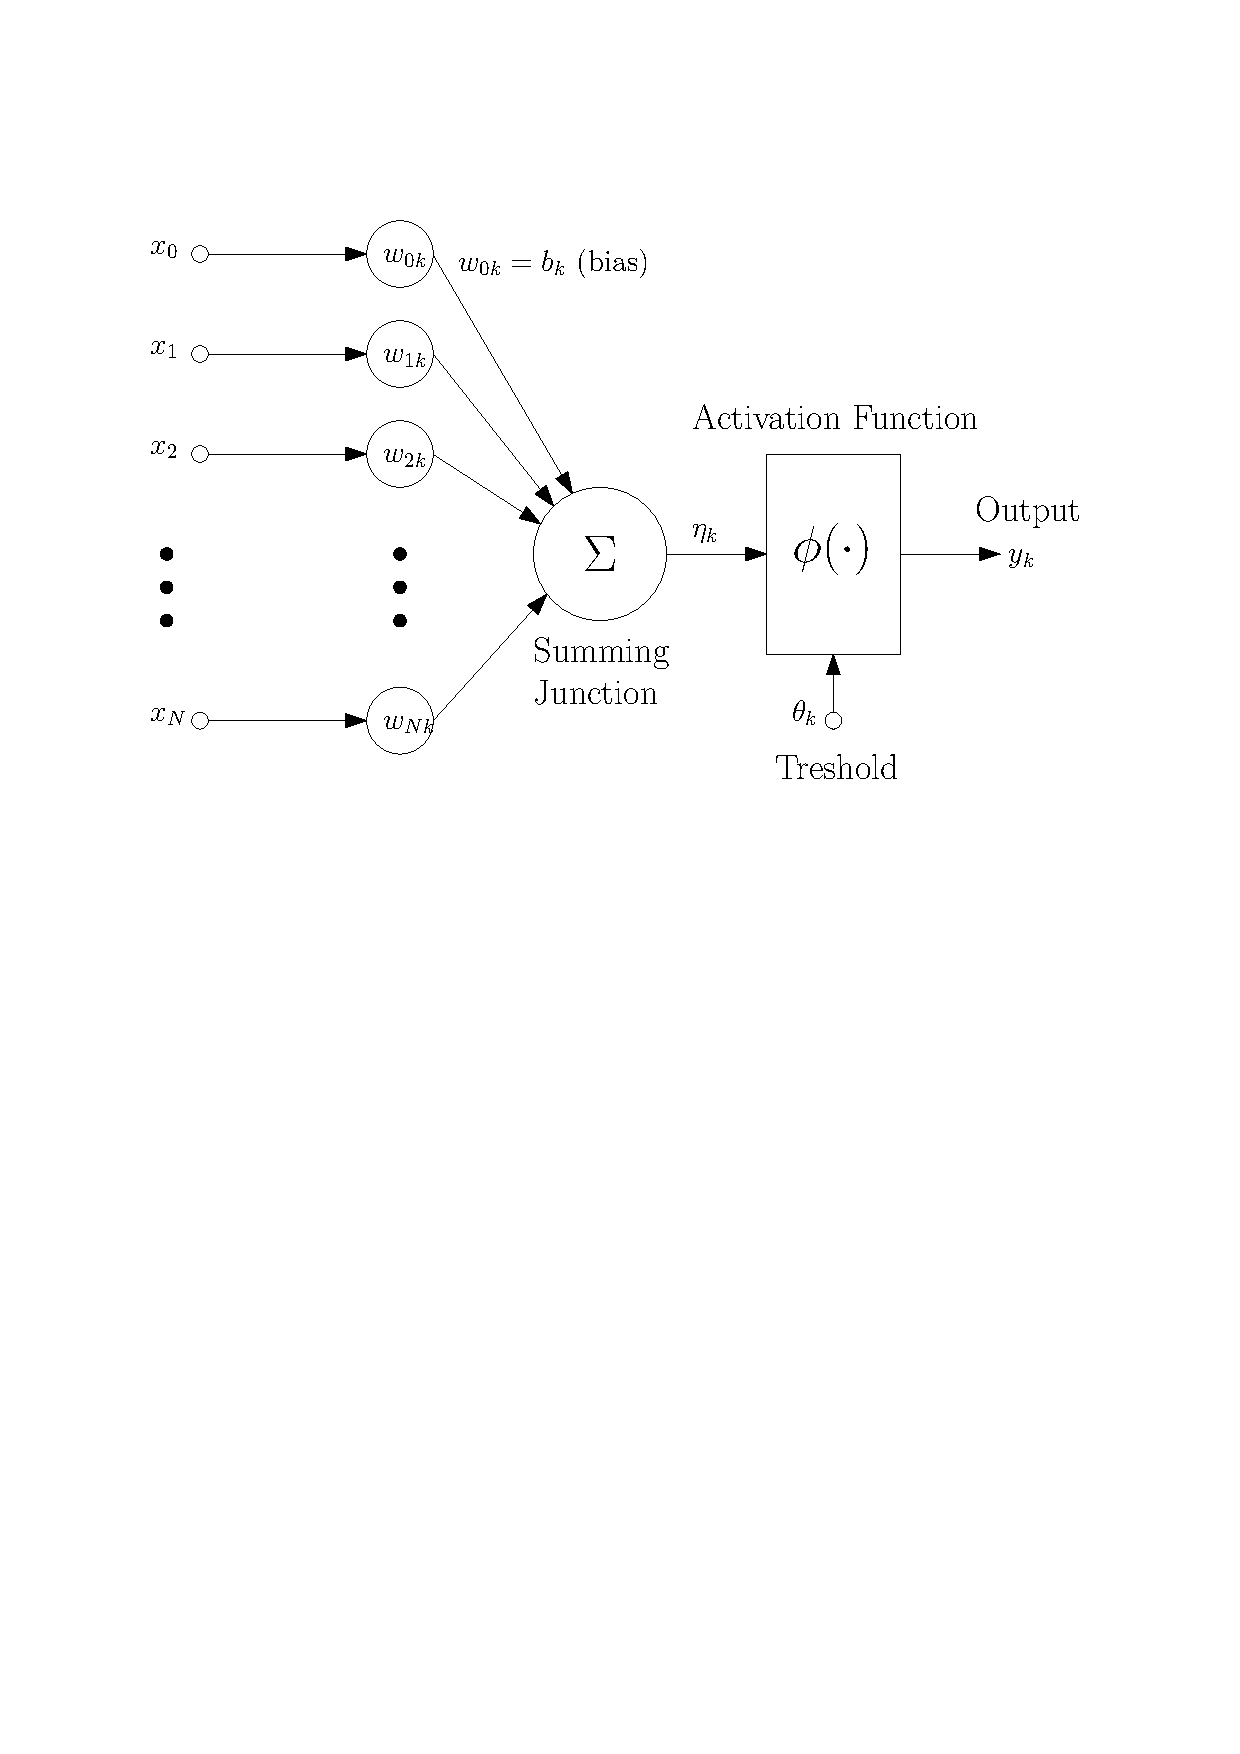
\includegraphics[width=0.9\textwidth]{img/perceptron.pdf}    
    \caption{Perceptrón (McCulloch a Pitts, 1943). Označenie: $x$ je \emph{vstupný vektor} pre ktorý $x_0=1$; $w_{\_k}$ je \emph{váhový vektor}; $\Sigma$ je \emph{sumačná funkcia}; $\eta_k$ je \emph{net}; $\phi$ je \emph{aktivačná funkcia}; $\theta_k$ je \emph{treshold}; $y_k$ je \emph{daný výstup} a $b_k$ je \emph{bias}.} 
    \label{fig:perceptron}
  \end{figure} 

\end{frame}

%========================================================================

\newcommand{\Bx}{{\bf x}}
\newcommand{\By}{{\bf y}}
\newcommand{\Bh}{{\bf h}}
\newcommand{\Bw}{{\bf w}}
\newcommand{\Bc}{{\bf c}}

%Bidirectional Activation-based Learning algorithm (BAL) shares with GeneRec
%the phase-based activations and unit types, but differs from it by the connectivity
%that allows completely bidirectional associations to be established (GeneRec
%focuses on input-to-output mapping). Unlike GeneRec, BAL uses two pairs of
%weight matrices for each activation phase. In addition, in BAL we do not use
%dynamical settling process but compute the activations in one step as described
%in Table 2.
\begin{frame}{Kontext práce - BAL}
  \begin{itemize}
    \item BAL $:=$ Bidirectional Activation-based Neural Network Learning Algorithm (Farkaš a Rebrová, 2013).
    \item Učenie závisí na rozdiely dopredných a spätných aktivácií. 
  \end{itemize}
  
  \begin{figure}[h!]  
    \centering
    \vspace{-5pt} 
    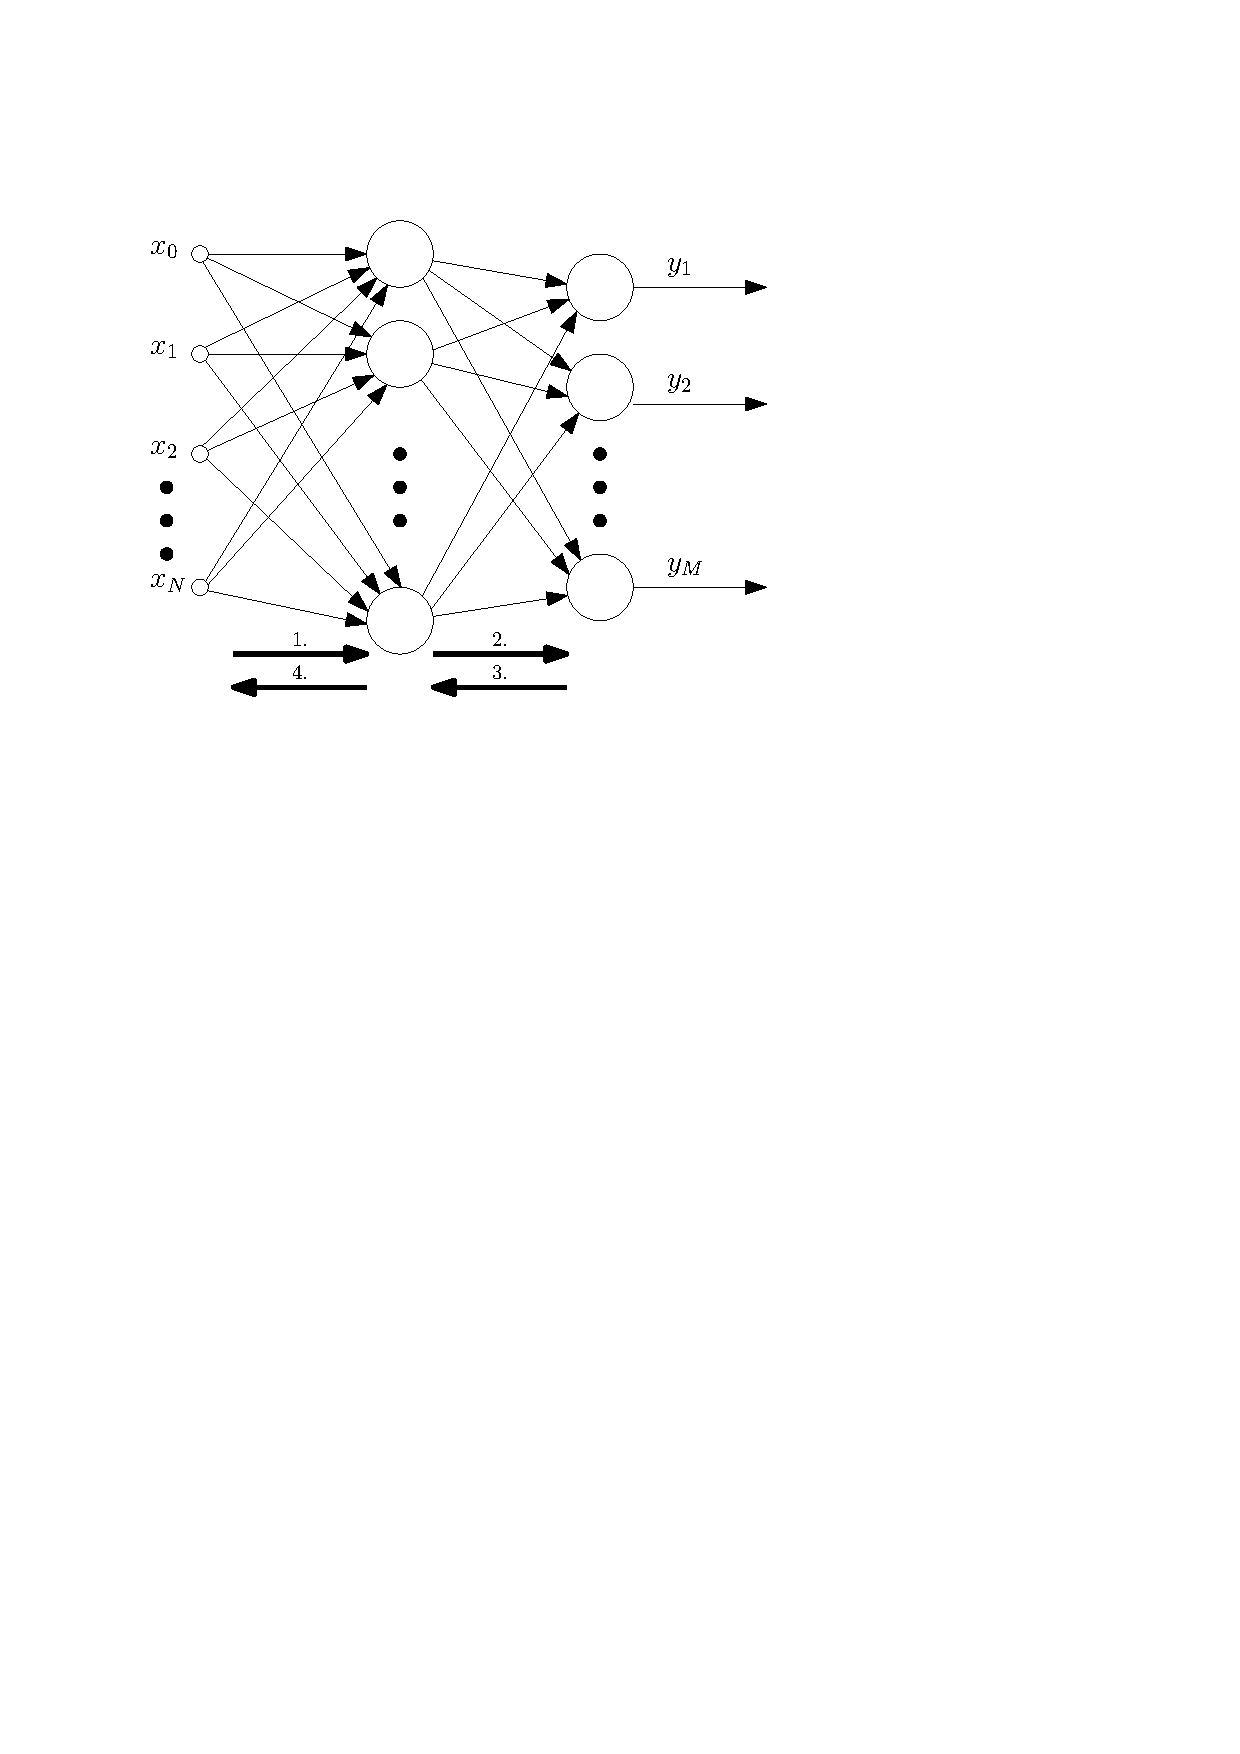
\includegraphics[scale=0.75]{img/bal.pdf}
    %\caption{{\tiny A standard 3-layer network (Wikipedia).}} 
  \end{figure} 
\end{frame}

\begin{frame}{Kontext práce - BAL}
  \begin{itemize} 
    \item BAL $:=$ Bidirectional Activation-based Neural Network Learning Algorithm (Farkaš a Rebrová, 2013).
    \item Učiace pravidlo: $ \frac{1}{\epsilon}\Delta w_{ik} = a_{i}^{-}(a_{k}^{+} - a_{k}^{-}). $
  \end{itemize} 

  \begin{table}
    \centering
    \begin{tabular}{|cccl|}
      \hline
      Vrstva & Fáza & Vstup & Aktivácia\\
      \hline
      $x$ & F & - & $x^{\rm F}_i$ = dopredný vstup\\ [1ex]
      $h$ & F & \hspace{0.3cm}$\eta^{\rm F}_j = \sum_i w_{ij}^{IH}x^{F}_i$\hspace{0.3cm} & $h^{\rm F}_j = \sigma(\eta^{\rm F}_j)$\hspace{0.3cm}\\ [1ex]
      $y$ & F & $\eta^{\rm F}_k = \sum_j w_{jk}^{HO}h^{F}_j$ & $y^{\rm F}_k = \sigma(\eta^{\rm F}_k)$\\ [1ex]
      \hline
      $y$ & B & - & $y^{\rm B}_k$ = spätný vstup\\ [1ex]
      $h$ & B & $\eta^{\rm B}_j = \sum_k w_{kj}^{OH}y^{\rm B}_k$ & $h^{\rm B}_j = \sigma(\eta^{\rm B}_j)$\\ [1ex]
      $x$ & B  & $\eta^{\rm B}_i = \sum_j w_{ji}^{HI}h^{\rm B}_j$ & $x^{\rm B}_i = \sigma(\eta^{\rm B}_i)$\\
      \hline
    \end{tabular}
    %\caption{Activation phases and states in the BAL model (Farkaš and Rebrová, 2013).}
    \label{tab:bal-states}
  \end{table}
\end{frame}

%%%%%%%%%%%%%%%%%%%%%%%%%%%%%%%%%%%%%%%%%%%%%%%%%%%%%%%%%%%%%%%%%%%%%%%%%
%%%%%%%%%%%%%%%%%%%%%%%%%%%%%%%%%%%%%%%%%%%%%%%%%%%%%%%%%%%%%%%%%%%%%%%%%
%V nadväznosti na úvodnú časť formulujte cieľ diplomovej práce.
%Na stránky uvádzajte malý počet riadkov.
%Vyhýbajte sa používaniu žargónu.
%Používajte starú múdrosť: 1 obrázok je viac než 1000 slov.
%%%%%%%%%%%%%%%%%%%%%%%%%%%%%%%%%%%%%%%%%%%%%%%%%%%%%%%%%%%%%%%%%%%%%%%%%
%%%%%%%%%%%%%%%%%%%%%%%%%%%%%%%%%%%%%%%%%%%%%%%%%%%%%%%%%%%%%%%%%%%%%%%%%

\begin{frame}{Cieľ diplomovej práce} 
  \begin{enumerate} 
    %\item Implement the GeneRec learning algorithm and test its properties using selected data sets.
    %\item Consider suitable modifications of the algorithm aimed at improving the network performance.
    %\item Analyse the convergence of the BAL network aimed at finding parameters on which the convergence depends. 
    \item Implementovať a analyzovať modely BAL a GeneRec. 
    \item Zvážiť vhodné modifikácie algoritmu zamerané na úspešnosť siete. 
    %\item Implementovať algoritmus GeneRec a porovnať ho s BALom. 
  \end{enumerate} 
  
  \begin{figure}[h!]  
    \centering
    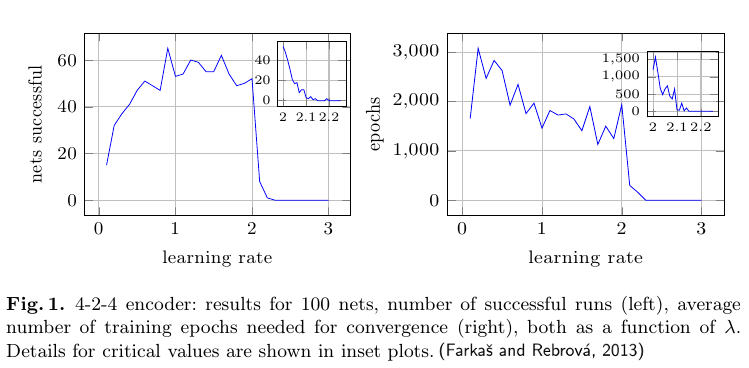
\includegraphics[scale=0.40]{img/bal_performance.png}
    \caption{\small 4-2-4 enkóder: výsledky pre 100 sietí, počet úspešných sietí~(vľavo), priemerný počet trénovacích epoch potrebných na konvergenciu~(vpravo), obe ako funkcie~$\lambda$. (Farkaš a Rebrová, 2013)} 
  \end{figure}  
  
\end{frame} 

%%%%%%%%%%%%%%%%%%%%%%%%%%%%%%%%%%%%%%%%%%%%%%%%%%%%%%%%%%%%%%%%%%%%%%%%%
%%%%%%%%%%%%%%%%%%%%%%%%%%%%%%%%%%%%%%%%%%%%%%%%%%%%%%%%%%%%%%%%%%%%%%%%%
%V ďalšej časti prezentujte vlastný prínos a vlastné výsledky porovnajte s výsledkami iných. Charakterizujte použité metódy.
%Na stránky uvádzajte malý počet riadkov.
%Vyhýbajte sa používaniu žargónu.
%Používajte starú múdrosť: 1 obrázok je viac než 1000 slov.
%%%%%%%%%%%%%%%%%%%%%%%%%%%%%%%%%%%%%%%%%%%%%%%%%%%%%%%%%%%%%%%%%%%%%%%%%
%%%%%%%%%%%%%%%%%%%%%%%%%%%%%%%%%%%%%%%%%%%%%%%%%%%%%%%%%%%%%%%%%%%%%%%%%

\begin{frame}{Vlastný prínos a vlastné výsledky}
  \begin{itemize}
    \item Navrhnutie a analýza modelu s rôznymi rýchlosťami učenia pre rôzne váhové matice.
    \item Zvýšenie pôvodnej úspešnosti siete BAL z 61\% na 94\%. 
  \end{itemize} 
  
  \begin{figure}[H]
    \centering
    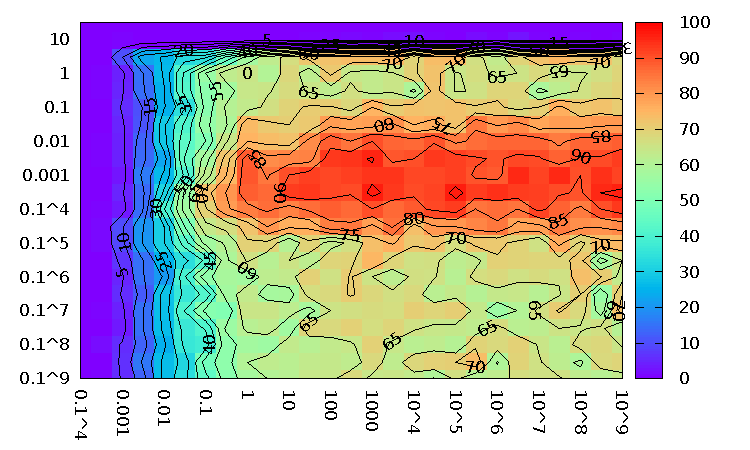
\includegraphics[width=0.54\textwidth]{../text/img/tlr-auto4-success.pdf}   
    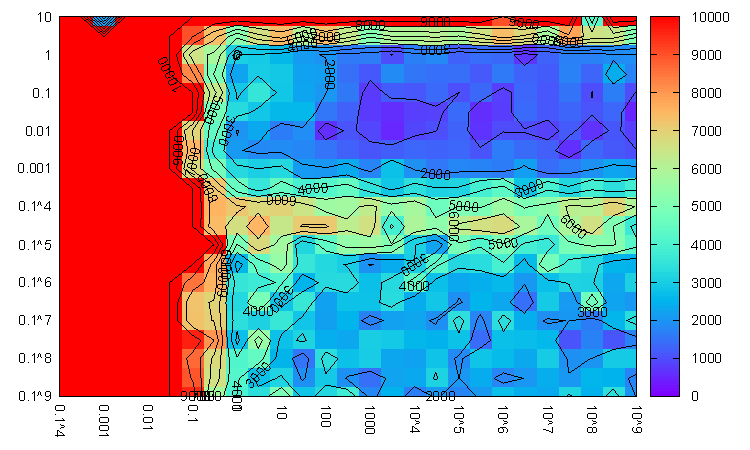
\includegraphics[width=0.54\textwidth]{../text/img/tlr-auto4-epoch.pdf}     
    %\caption{TLR success rate and convergence time needed for successful networks on the \emph{4-2-4 encoder} task with $\sigma = 2.3$ and $\mu = 0.0$. Best network achieved $96.5\$$ with $\lambda_h=0.0003$ and $\lambda_v=1000.0$.}
    \label{fig:results-tlr-auto4-performance}
  \end{figure}
\end{frame}

\begin{frame}{Vlastný prínos a vlastné výsledky}
  \begin{itemize}
%    \item Zrekonštruovanie výsledkov GeneRec a BAL. 
    \item Analýza atribútov siete BAL v priebehu učenia. 
    \item Zvýšenie úspešnosti pri výbere sietí so vzdialenejšími reprezentáciami na skrytej vrstve (99.86\%). 
  \end{itemize} 
  
  \begin{figure}[h!]  
    \centering
    \vspace{-8pt} 
    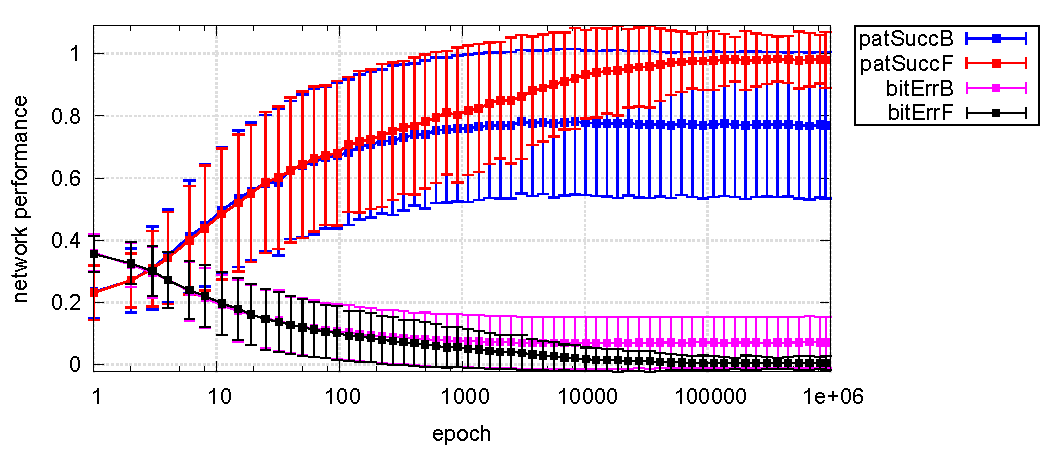
\includegraphics[width=0.65\textwidth]{../text/img/tlr-auto4-best-perf.pdf}\\
    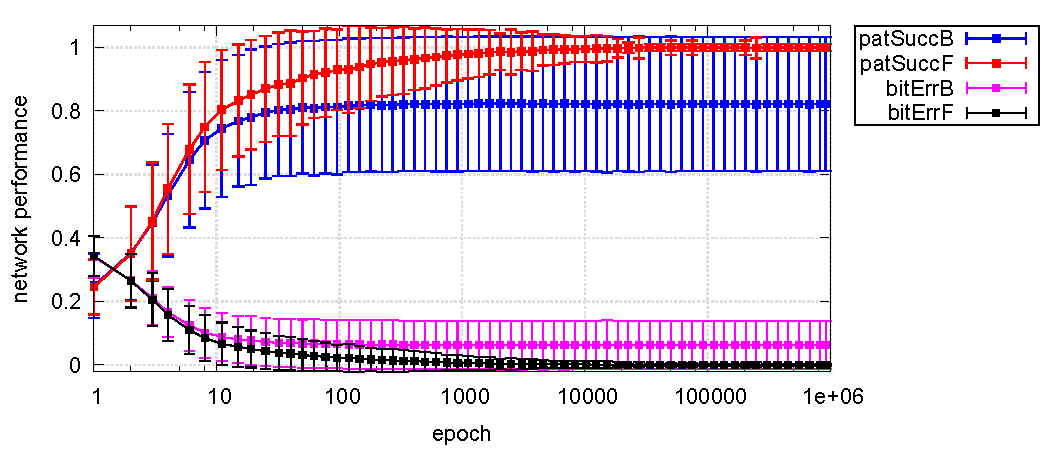
\includegraphics[width=0.65\textwidth]{../text/img/tlr-auto4-best-can.pdf}    
  %  \caption{{\tiny $\lambda = \epsilon$ = rýchlosť učenia; $\sigma$ = disperzia normálnej distribúcie pôvodných váh}} 
  \end{figure} 
\end{frame}


%TODO legenda ku grafom 

\begin{frame}{Porovnanie s výsledkami iných}
  \begin{table}[H] 
    \centering
      \begin{tabular}{|l|l|l|l|l|}
      \hline
      Model &$\lambda_h$&$\lambda_v$&$patSucc^F$ &Epochy\\ %&SEM(success) \\
      \hline
      BP&2.4 &2.4 &100\%&60\\ %&5.1\\
      \hline
      GR&0.6 &0.6 &90\%&418\\ %&28\\
      \hline
      GR Sym&1.4 &1.4 &56\%&88\\ %&2.9\\
      \hline
      GR Mid&2.4 &2.4 &92\%&60\\ %&3.4\\
      \hline
      CHL&1.2 &1.2 &56\%&77\\ %&1.8\\
      \hline
      BAL&0.9 &0.9 &62.7\%& 5136.11\\ %&2.0e+08\\
      \hline
      {\bf BAL TLR}&0.0002  & 500&93.12\%&5845.01\\ %&1.52e+08\\
      \hline
      {\bf BAL TLR Can}&0.0002&500&99.86\%&150.417\\ %&5,070,000\\
      \hline
      {\bf BAL Recirc}&0.0001&1.0&36\%&1221.6\\ %&4.31e+07\\
      \hline
      {\bf BAL GLR}& any & any & 0\% & N/A \\
      \hline 
      \end{tabular}
    \caption{Výsledky pre 4-2-4 enkóder. BP, GR, GR Sym, GR Mid a CHL prebraté z (O'Reilly,~1996)} 
  \label{tab:results-cmp-auto4}
\end{table}
\end{frame}

\begin{frame}{Použité metódy - čo nefungovalo}
  \begin{itemize}
    %\item Vyskúšali sme viacero variantov siete BAL: 
    %\begin{itemize} 
      \item Iné učiace pravidlá, napr. pravidlo CHL {\tiny (Movellan, 1990)}.
      \item Moment učenia. Dávkové učenie. Permutácia vstupov. 
      \item Vynechanie niektorých skrytých neurónov {\tiny (Dropout, Hinton, 2012)}. 
      \item Pridanie recirkulácie. Pridanie šumu.
      \item Dynamická rýchlosť učenia {\tiny (Yu a Chen, 1997)}. 
      \item Symetrické váhy. 
      \item Iné.
      \item Kombinácie predošlých. 
%      \item Cielené generovanie počiatočných váh. 
    %\end{itemize} 
    %\item V prípade 4-2-4 enkódera-a sme dosiahli 94\% úspešnosť, pričom Backpropagation má 100\% úspešnosť (jednosmerne). 
  \end{itemize} 
\end{frame} 

\begin{frame}{Analýza siete BAL - Zobrazenie priebehu}
  \begin{figure}[h!]  
    \centering
    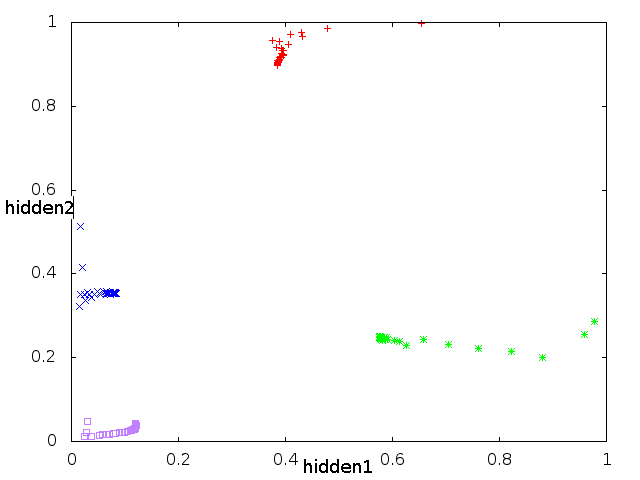
\includegraphics[scale=0.4]{img/nice.png}
    \caption{{\small Zobrazenie priebehu skrytých aktivácií. Táto sieť bola {\bf úspešná}.}} 
  \end{figure} 
\end{frame} 

\begin{frame}{Analýza siete BAL - Zobrazenie priebehu}
  \begin{figure}[h!]  
    \centering
    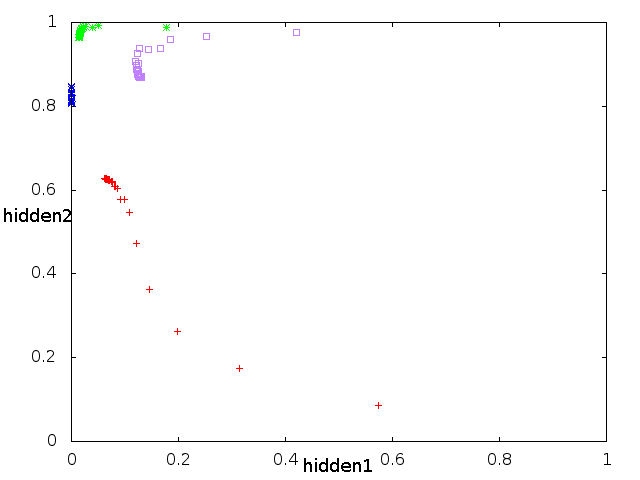
\includegraphics[scale=0.4]{img/left_top.png}
    \caption{{\small Zobrazenie priebehu skrytých aktivácií. Táto sieť bola {\bf úspešná}.} }
  \end{figure} 
\end{frame}

\begin{frame}{Analýza siete BAL - Zobrazenie priebehu}
  \begin{figure}[h!]  
    \centering
    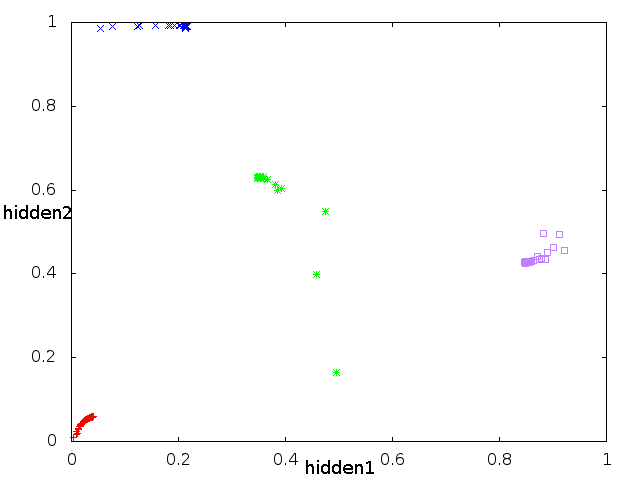
\includegraphics[scale=0.4]{img/tazisko.png}
    \caption{{\small Zobrazenie priebehu skrytých aktivácií. Táto sieť bola {\bf neúspešná}.} }
  \end{figure} 
\end{frame}

\begin{frame}{Analýza siete BAL - Zobrazenie priebehu}
  \begin{figure}[h!]  
    \centering
    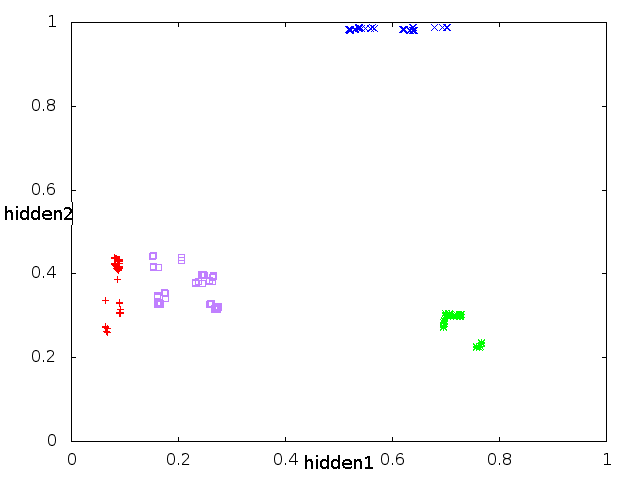
\includegraphics[scale=0.4]{img/non-convergent.png}
    \caption{{\small Zobrazenie priebehu skrytých aktivácií. Táto sieť bola {\bf neúspešná}.}} 
  \end{figure} 
\end{frame}


\begin{frame}{Analýza siete BAL - Spätné zobrazenie cifier}
  \begin{itemize} 
    \item Trénovací súbor \emph{Cifry} pozostáva z 42000 obrázkov $28 \times 28$ rukou napísaných cifier. 
  \end{itemize} 

  \begin{table}[H] 
    \centering
      \begin{tabular}{|l|l|l|l|l|}
      \hline
      Model&$\lambda_h$&$\lambda_v$&$patSucc^F$ &Epochy\\ %&SEM(success) \\
      \hline
      Lineárny klasifikátor & -- & -- & 88 & -- \\ 
      \hline
      BP 784--300--10& -- & -- & 95.3 & -- \\ 
      %\hline 
      %BAL 784--300--10~(\ref{sec:models-bal})& 0.01 & 0.01 & 9.8 & 20 \\
      \hline 
      TLR 784--300--10& $10^{-8}$ & 0.1 & 88.47 & 20 \\
      \hline 
      GeneRec 784--300--50--10& 0.03 & 0.03 & 43.22 & 50 \\
      \hline 
      \end{tabular}
    \caption{Výsledky pre LK a BP prevzaté z LeCun (1998).} 
    \label{tab:results-cmp-digits}
  \end{table}

  %TODO preblikavanie na originalne 
  \begin{figure}[H]
    \centering
    
\includegraphics[width=0.7\textwidth]{img/tlr-digits.png}  
  \end{figure}   

\end{frame}

%%%%%%%%%%%%%%%%%%%%%%%%%%%%%%%%%%%%%%%%%%%%%%%%%%%%%%%%%%%%%%%%%%%%%%%%%
%%%%%%%%%%%%%%%%%%%%%%%%%%%%%%%%%%%%%%%%%%%%%%%%%%%%%%%%%%%%%%%%%%%%%%%%%
%Na záver sformulujte možnosti ďalšieho rozpracovania práce.
%Na stránky uvádzajte malý počet riadkov.
%Vyhýbajte sa používaniu žargónu.
%Používajte starú múdrosť: 1 obrázok je viac než 1000 slov.
%%%%%%%%%%%%%%%%%%%%%%%%%%%%%%%%%%%%%%%%%%%%%%%%%%%%%%%%%%%%%%%%%%%%%%%%%
%%%%%%%%%%%%%%%%%%%%%%%%%%%%%%%%%%%%%%%%%%%%%%%%%%%%%%%%%%%%%%%%%%%%%%%%%

\begin{frame}{Možnosti ďalšieho rozpracovania práce}
  \begin{itemize} 
    \item Inicializácia váh s určitými vlastnosťami.
    \item Rozšírenie myšlienky dvoch rýchlostí učenia na ďalšie modely neurónových sietí.  
    \item Zrýchlenie učiacej fázy. 
    \item Matematická formulácia aproximácie dynamického systému siete BAL a skúmanie jeho konvergencie. 
  \end{itemize} 
\end{frame} 

\begin{frame}{Ďakujem za pozornosť!}
  \begin{center}
{\bf Ďakujem za pozornosť!} 
  \end{center}
  
  \vspace{2cm}
  
  \begin{center}
  \url{https://github.com/Petrzlen/master_thesis} \\
  \vspace{5mm} 
  %\small{P.S. Ospravedlňujeme sa za kvalitu obrázkov (TODO pdf).}
  \end{center}
\end{frame}

\begin{frame}{Pripomienky oponenta}
  \begin{itemize} 
    \item Máte to celé zle. 
  \end{itemize} 
\end{frame} 

\end{document}

